% ----------------------------------------------------------------------------
% CONSTRUTOR E DESTRUTOR
% ----------------------------------------------------------------------------

\chapter{Construtor e destrutor}

O Construtor de um objeto pode receber parâmetros. Estes parâmetros são
ilustrados abaixo.

\begin{figure}[h!]
	\centering
	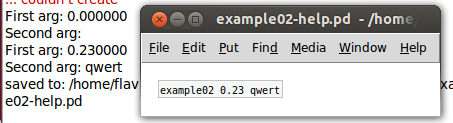
\includegraphics[width=0.7\textwidth]{example2}
	\caption{External recebendo parâmetros. Note a tela de saída no fundo da imagem.}
\end{figure}

\section{Construtor}

Parâmetros de inicialização no construtor podem permitir que inicializemos o
external com determinados valores. Isto é feito definindo os parâmetros no
métodos class\_new() quanto na definição da função construtora. (Veja o
exemplo02).

\begin{lstlisting}

// Constructos of the class
void * example2_new(t_symbol * arg1, t_floatarg arg2) {
    t_example2 *x = (t_example2 *) pd_new(example2_class);
    post("First arg: %s", arg1->s_name);
    post("Second arg: %f", arg2);
    return (void *) x;
}

void example2_setup(void) {
    example2_class = class_new(gensym("example2"),
            (t_newmethod) example2_new, // Constructor
            0,
            sizeof (t_example2),
	    CLASS_NOINLET,
            A_DEFFLOAT, // First Constructor parameter
            A_DEFSYMBOL, // Second Consctructo parameter
            0);
}
\end{lstlisting}

Notem que os parâmetros são definidos com um tipo e são recebidos com outro.
São tipos padrões do Pure Data. Estes tipos são chamados atom e alguns estão
documentados no tutorial do IOHannes. Eles são:

\begin{itemize}
\item A\_NULL,
\item A\_FLOAT,
\item A\_SYMBOL,
\item A\_POINTER,
\item A\_SEMI,
\item A\_COMMA,
\item A\_DEFFLOAT,
\item A\_DEFSYM,
\item A\_DOLLAR, 
\item A\_DOLLSYM,
\item A\_GIMME,
\item A\_CANT
\end{itemize}
(Retirado do arquivo m\_pd.h)

*** Nunca usei todos eles. Pra que será que servem?

Entre estes tipos, um deles pode aceitar qualquer quantidade e tipo de
parâmetros. É o A\_GIMME. (Veja o exemplo09). 

\begin{lstlisting}

// Constructos of the class
void * example9_new(t_symbol *s, int argc, t_atom * argv) {
    t_example9 *x = (t_example9 *) pd_new(example9_class);
    post("%d parameters received",argc);
    return (void *) x;
}


void example9_setup(void) {
    example9_class = class_new(gensym("example9"),
            (t_newmethod) example9_new, // Constructor
            (t_method) example9_destroy, // Destructor
            sizeof (t_example9),
	    CLASS_NOINLET,
	    A_GIMME, // Allows various parameters
            0); // LAST argument is ALWAYS zero
}
\end{lstlisting}

Quando utilizamos o A\_GIMME a função construtora trabalha como um programa
main em C. Recebe os parâmetros argv e argc, um com uma lista de atoms e outro
com a quantidade de atoms nesta lista.

\begin{figure}[h!]
	\centering
	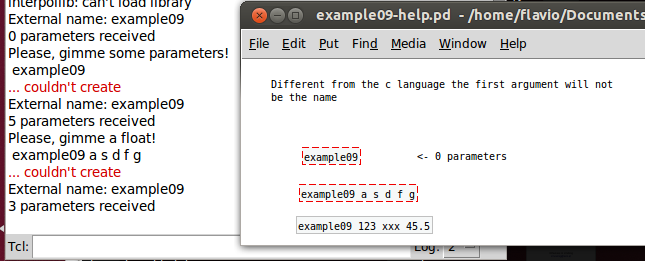
\includegraphics[width=0.7\textwidth]{example9}
	\caption{Diferente da linguagem C, o primeiro parâmetro não é o nome do external.}
\end{figure}

Note que o Pure Data não obriga que o usuário passe parâmetros para o objeto. É
como se todo construtor, independentemente de como ele está definido, aceitasse
sua instanciação vazia. Cabe ao programador verificar se os parâmetros
recebidos são em quantidade, tipo e valor esperado e, caso não seja, abortar a
construção do objeto e não retornar sua instância.

\section{Destrutor}
O destrutor de uma classe permite liberar a memória do Pure Data dos dados que foram alocados. (Veja o exemplo07)
\begin{lstlisting}
// Destroy the class
void example9_destroy(t_example9 *x) {
   post("You say good bye and I say hello");
}

void example9_setup(void) {
    example9_class = class_new(gensym("example9"),
            (t_newmethod) example9_new, // Constructor
            (t_method) example9_destroy, // Destructor
            sizeof (t_example9),
	    CLASS_NOINLET,
	    A_GIMME, // Allows various parameters
            0); // LAST argument is ALWAYS zero
}

\end{lstlisting}

A liberação da memória pode ser feita com a função freebytes() definida na API
do Pure Data.

\begin{lstlisting}
void freebytes(void *x, size_t nbytes)
\end{lstlisting}

